\documentclass[12pt,letterpaper]{article}
\usepackage{graphicx,textcomp}
\usepackage{natbib}
\usepackage{setspace}
\usepackage{fullpage}
\usepackage{color}
\usepackage[reqno]{amsmath}
\usepackage{amsthm}
\usepackage{fancyvrb}
\usepackage{amssymb,enumerate}
\usepackage[all]{xy}
\usepackage{endnotes}
\usepackage{lscape}
\newtheorem{com}{Comment}
\usepackage{float}
\usepackage{hyperref}
\newtheorem{lem} {Lemma}
\newtheorem{prop}{Proposition}
\newtheorem{thm}{Theorem}
\newtheorem{defn}{Definition}
\newtheorem{cor}{Corollary}
\newtheorem{obs}{Observation}
\usepackage[compact]{titlesec}
\usepackage{dcolumn}
\usepackage{tikz}
\usetikzlibrary{arrows}
\usepackage{multirow}
\usepackage{xcolor}
\newcolumntype{.}{D{.}{.}{-1}}
\newcolumntype{d}[1]{D{.}{.}{#1}}
\definecolor{light-gray}{gray}{0.65}
\usepackage{url}
\usepackage{listings}
\usepackage{color}

\definecolor{codegreen}{rgb}{0,0.6,0}
\definecolor{codegray}{rgb}{0.5,0.5,0.5}
\definecolor{codepurple}{rgb}{0.58,0,0.82}
\definecolor{backcolour}{rgb}{0.95,0.95,0.92}

\lstdefinestyle{mystyle}{
	backgroundcolor=\color{backcolour},   
	commentstyle=\color{codegreen},
	keywordstyle=\color{magenta},
	numberstyle=\tiny\color{codegray},
	stringstyle=\color{codepurple},
	basicstyle=\footnotesize,
	breakatwhitespace=false,         
	breaklines=true,                 
	captionpos=b,                    
	keepspaces=true,                 
	numbers=left,                    
	numbersep=5pt,                  
	showspaces=false,                
	showstringspaces=false,
	showtabs=false,                  
	tabsize=2
}
\lstset{style=mystyle}
\newcommand{\Sref}[1]{Section~\ref{#1}}
\newtheorem{hyp}{Hypothesis}

\title{Problem Set 2}
\date{Due: October 22, 2026}
\author{Elena Gyubin Lee}

\begin{document}
	\maketitle
	\section*{Instructions}
\begin{itemize}
	\item Please show your work! You may lose points by simply writing in the answer. If the problem requires you to execute commands in \texttt{R}, please include the code you used to get your answers. Please also include the \texttt{.R} file that contains your code. If you are not sure if work needs to be shown for a particular problem, please ask.
	\item Your homework should be submitted electronically on GitHub.
	\item This problem set is due before 23:59 on Thursday October 22, 2026. No late assignments will be accepted.

\end{itemize}

	
	\vspace{.5cm}
	\section*{Question 1: Political Science}
		\vspace{.25cm}
	The following table was created using the data from a study run in a major Latin American city.\footnote{Fried, Lagunes, and Venkataramani (2010). ``Corruption and Inequality at the Crossroad: A Multimethod Study of Bribery and Discrimination in Latin America. \textit{Latin American Research Review}. 45 (1): 76-97.} As part of the experimental treatment in the study, one employee of the research team was chosen to make illegal left turns across traffic to draw the attention of the police officers on shift. Two employee drivers were upper class, two were lower class drivers, and the identity of the driver was randomly assigned per encounter. The researchers were interested in whether officers were more or less likely to solicit a bribe from drivers depending on their class (officers use phrases like, ``We can solve this the easy way'' to draw a bribe). The table below shows the resulting data.

\newpage
\begin{table}[h!]
	\centering
	\begin{tabular}{l | c c c }
		& Not Stopped & Bribe requested & Stopped/given warning \\
		\\[-1.8ex] 
		\hline \\[-1.8ex]
		Upper class & 14 & 6 & 7 \\
		Lower class & 7 & 7 & 1 \\
		\hline
	\end{tabular}
\end{table}

\begin{enumerate}
	
	\item [(a)]
	\textbf{Calculate the $\chi^2$ test statistic by hand/manually (even better if you can do "by hand" in \texttt{R}).}\\
	
	\noindent First, I saved the observed frequencies as a matrix and calculated the row, column and grand totals.
	\lstinputlisting[language=R, firstline=37, lastline=59]{PS02_answers_EGL.R}
	
	Expected frequencies are $f_e = \frac{\text{row total }\times\text{ column total}}{\text{grand total}}$.
	\lstinputlisting[language=R, firstline=61, lastline=77]{PS02_answers_EGL.R}
	\begin{verbatim}
	       Outcome
	Class   Not Stopped Bribe Requested Stopped/Warned
	Upper        13.5        8.357143       5.142857
	Lower         7.5        4.642857       2.857143
	\end{verbatim}
	As noted in the footnote, two expected counts fall below 5 (4.64 and 2.86) and one is barely above (5.14), so the $\chi^2$ approximation is somewhat shaky.
	
	\lstinputlisting[language=R, firstline=82, lastline=85]{PS02_answers_EGL.R}
	\begin{verbatim}
		[1] 3.791168
	\end{verbatim}
	
	\item [(b)]
	\textbf{Now calculate the p-value from the test statistic you just created (in \texttt{R}).\footnote{Remember frequency should be $>$ 5 for all cells, but let's calculate the p-value here anyway.}  What do you conclude if $\alpha = 0.1$?}\\
	
	\noindent Degrees of freedom are $(r-1)(c-1) = 2$. The $\chi^2$ distribution is right-skewed, so we use the upper tail.
	
	\lstinputlisting[language=R, firstline=89, lastline=95]{PS02_answers_EGL.R}
	
	We can check our numbers by comparing it with the default R function output.
	
	\lstinputlisting[language=R, firstline=97, lastline=98]{PS02_answers_EGL.R}
	\begin{verbatim}
		chisq = 3.791168, df = 2, p_val = 0.1502306
		X-squared = 3.7912, df = 2, p-value = 0.1502
	\end{verbatim}
	
	\lstinputlisting[language=R, firstline=103, lastline=105]{PS02_answers_EGL.R}
		\begin{verbatim}
		[1] FALSE
	\end{verbatim}
	To conclude, since $p = 0.150 > 0.1$, we fail to reject $H_0$. There is insufficient evidence at the 10\% level that social class and the outcome of police encounters are associated.
	\vspace{1cm}
	
	\item [(c)] \textbf{Calculate the standardized residuals for each cell and put them in the table below.}
	\vspace{0.5cm}
	
	Like any test statistic, a standardised residual takes the form (observed $-$ expected under the null) divided by a standard error. For each cell, the observed value is $f_o$, the null expectation is $f_e$, and the standard error is $\sqrt{f_e\,(1-\text{row prop.})(1-\text{column prop.})}$, so that
	
	\[
	z = \frac{f_o - f_e}{\sqrt{f_e\,(1-\text{row prop.})(1-\text{column prop.})}}.
	\] 
	
	This expresses each cell's distance from independence in standard-error units, which makes the cells comparable with one another.
	
	\lstinputlisting[language=R, firstline=114, lastline=132]{PS02_answers_EGL.R}
	\begin{verbatim}
					Outcome
		Class   Not Stopped Bribe Requested Stopped/Warned
		Upper   0.3220306       -1.641957       1.523026
		Lower  -0.3220306        1.641957      -1.523026
	\end{verbatim}
	
	
	I checked that the results match R's built-in function.
	\lstinputlisting[language=R, firstline=134, lastline=135]{PS02_answers_EGL.R}
	
	\begin{table}[h]
		\centering
		\begin{tabular}{l | c c c }
			& Not Stopped & Bribe requested & Stopped/given warning \\
			\\[-1.8ex] 
			\hline \\[-1.8ex]
			Upper class  & 0.3220306 & -1.641957 & 1.523026  \\
			\\
			Lower class & -0.3220306 & 1.641957  & -1.523026  \\
			
		\end{tabular}
	\end{table}
	
	\vspace{1cm}
	\item [(d)] \textbf{How might the standardized residuals help you interpret the results?}  
		\vspace{0.5cm}
	
	\noindent The overall $\chi^2$ test tells us \emph{whether} class and outcome are dependent, but not \emph{where} any departure from independence lies. Standardized residuals answer that, since under $H_0$ they are approximately standard normal and can be compared cell by cell with a critical value. For $\alpha = 0.1$ the critical value is $|z| = 1.645$ (\texttt{qnorm(0.95)}). Because there are only two rows, the residuals in the two rows mirror each other.
	
	No cell reaches the 1.645 cutoff, which is consistent with our failure to reject $H_0$ in part (b). Two cells narrowly miss it:
	\begin{itemize}
		\item \textbf{Bribe requested} ($|z| = 1.642$): officers solicit bribes less often than expected from upper-class drivers and more often than expected from lower-class drivers.
		\item \textbf{Stopped/given warning} ($|z| = 1.523$): the pattern reverses. Upper-class drivers are stopped or warned more often than expected, and lower-class drivers less often.
	\end{itemize}
	
	Finally, the \textbf{Not stopped} column is almost exactly as expected under independence ($|z| = 0.322$).
	
	These patterns weakly suggest class-based differences in how officers behave, but they are not statistically significant at $\alpha = 0.1$. 
	
\end{enumerate}
\newpage

\section*{Question 2: Economics}
Chattopadhyay and Duflo were interested in whether women promote different policies than men.\footnote{Chattopadhyay and Duflo. (2004). ``Women as Policy Makers: Evidence from a Randomized Policy Experiment in India. \textit{Econometrica}. 72 (5), 1409-1443.} Answering this question with observational data is pretty difficult due to potential confounding problems (e.g. the districts that choose female politicians are likely to systematically differ in other aspects too). Hence, they exploit a randomized policy experiment in India, where since the mid-1990s, $\frac{1}{3}$ of village council heads have been randomly reserved for women. A subset of the data from West Bengal can be found at the following link: \url{https://raw.githubusercontent.com/kosukeimai/qss/master/PREDICTION/women.csv}\\

\noindent Each observation in the data set represents a village and there are two villages associated with one GP (i.e. a level of government is called "GP"). Figure~\ref{fig:women_desc} below shows the names and descriptions of the variables in the dataset. The authors hypothesize that female politicians are more likely to support policies female voters want. Researchers found that more women complain about the quality of drinking water than men. You need to estimate the effect of the reservation policy on the number of new or repaired drinking water facilities in the villages.
\vspace{.5cm}
\begin{figure}[h!]
	\caption{\footnotesize{Names and description of variables from Chattopadhyay and Duflo (2004).}}
	\vspace{.5cm}
	\centering
	\label{fig:women_desc}
	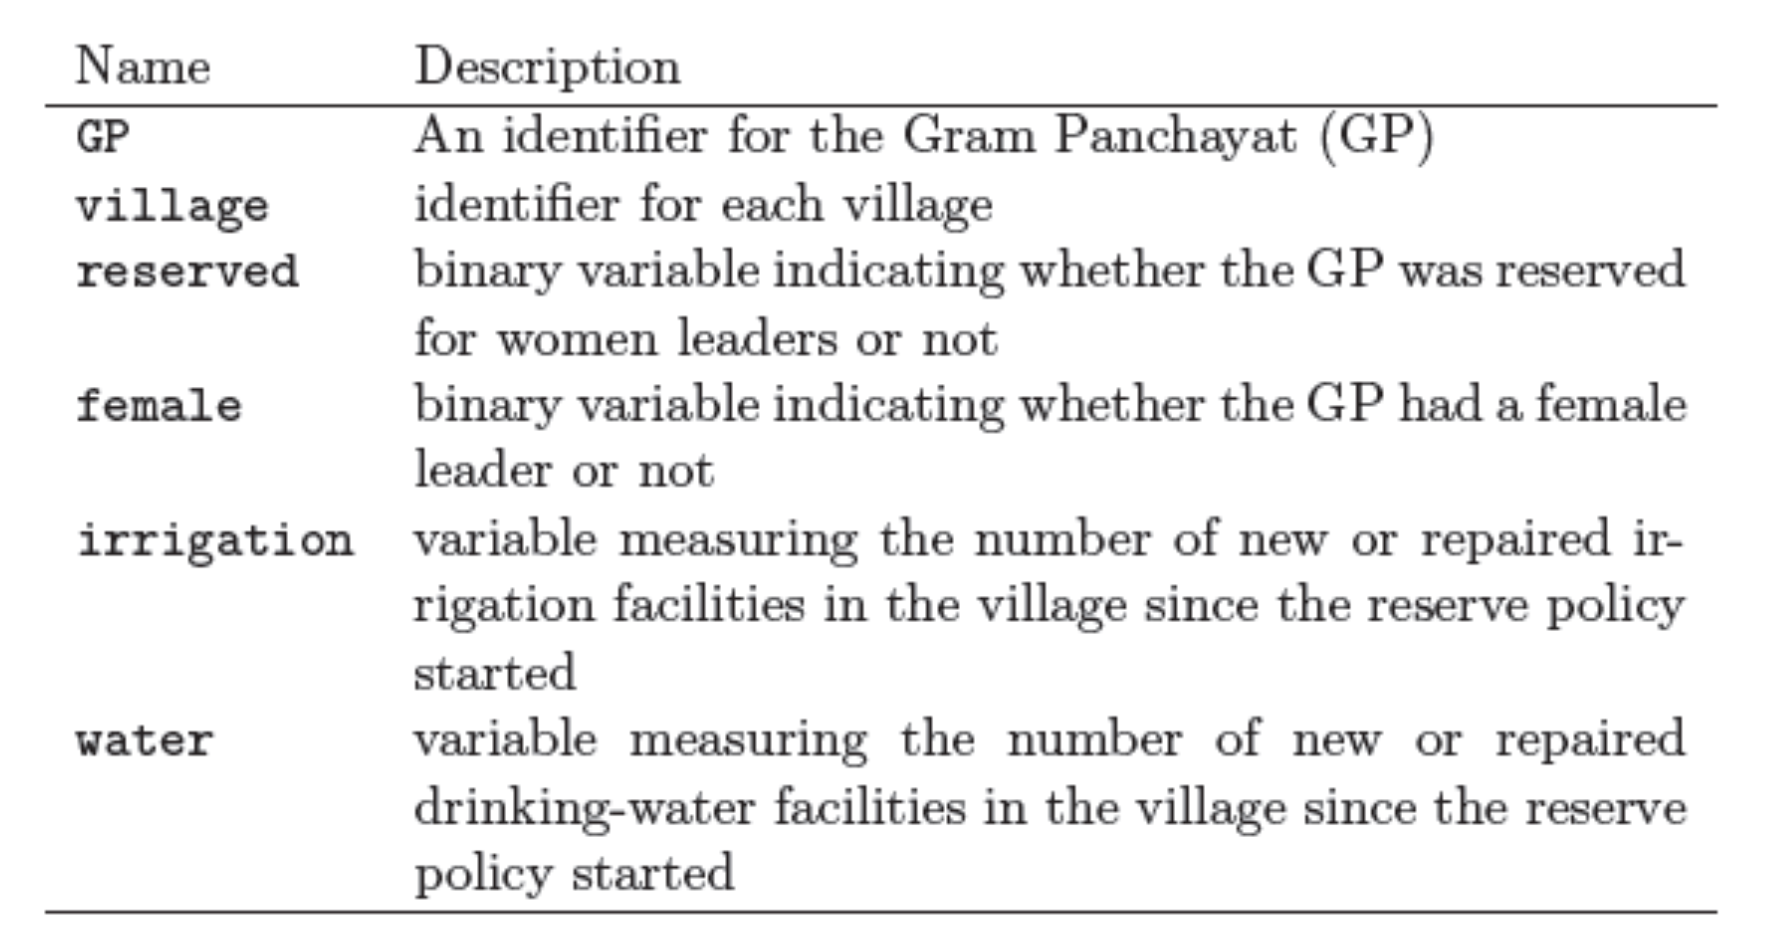
\includegraphics[width=.85\textwidth]{Figure1.png}
\end{figure}		

\newpage

\begin{enumerate}
	
	\item [(a)] \textbf{State a null and alternative (two-tailed) hypothesis.}\\
	
	Before anything, we load in the data and save it as a table called 'experiment'.
	\lstinputlisting[language=R, firstline=165, lastline=167]{PS02_answers_EGL.R}	
	
	These are some of the assumptions of this test.
	\begin{itemize}
		\item \textbf{Type of data:} the outcome (number of new or repaired drinking water \texttt{facilities}) is quantitative, and the explanatory variable (\texttt{reserved}) is binary.
		\item \textbf{Sampling:} the reservation of council head seats for women was randomly assigned, so the two groups of villages should be comparable on average.
		\item \textbf{Sample size:} the sample is much larger than 30, so theoretically (under the Central Limit Theorem) the sampling distribution of the mean is approximately normal.
	\end{itemize}
	\vspace{.3cm}
	
	\noindent Since the authors ask whether the reservation policy has an effect in \emph{either} direction, we use a two-tailed test. In the bivariate model $water_i = \beta_0 + \beta_1\,reserved_i + \epsilon_i$, the slope $\beta_1$ is the difference in the average number of facilities between reserved and unreserved villages. Thus the hypotheses are:\\
	
	\noindent \textbf{$H_0: \beta_1 = 0$ \quad (villages with and without a reservation policy build or repair the same number of drinking water facilities, on average).\\
	$H_A: \beta_1 \neq 0$ \quad (villages with and without a reservation policy do not build or repair the same number of drinking water facilities, on average).\\}
	\vspace{.5cm}
	
	\item [(b)] \textbf{Run a bivariate regression to test this hypothesis in \texttt{R} (include your code!).}
	\lstinputlisting[language=R, firstline=200, lastline=201]{PS02_answers_EGL.R}
	\begin{verbatim}
		Call:
		lm(formula = water ~ reserved, data = experiment)
		
		Residuals:
		Min      1Q  Median      3Q     Max 
		-23.991 -14.738  -7.865   2.262 316.009 
		
		Coefficients:
		Estimate Std. Error t value Pr(>|t|)    
		(Intercept)   14.738      2.286   6.446 4.22e-10 ***
		reserved       9.252      3.948   2.344   0.0197 *  
		---
		Signif. codes:  0 ‘***’ 0.001 ‘**’ 0.01 ‘*’ 0.05 ‘.’ 0.1 ‘ ’ 1
		
		Residual standard error: 33.45 on 320 degrees of freedom
		Multiple R-squared:  0.01688,	Adjusted R-squared:  0.0138 
		F-statistic: 5.493 on 1 and 320 DF,  p-value: 0.0197
	\end{verbatim}
	
	\vspace{.5cm}
	\item [(c)] \textbf{Interpret the coefficient estimate for reservation policy.}\\
	
	\noindent The coefficient estimate for the reservation policy is $9.252$, indicating that villages with a reservation policy built or fixed, on average, approximately $9.25$ more water facilities than villages without a reservation policy. Specifically, the predicted average number of water facilities built is $14.738$ in villages without a reservation policy and $14.738 + 9.252 = 23.990$ in villages with a reservation policy. This difference is statistically significant at the $5\%$ level ($p = 0.0197$).
	
	\noindent In addition to the slope coefficient, the full regression output provides several key parameters for interpretation:
	\begin{itemize}
		\item \textbf{Standard Error ($\text{SE} = 3.948$):} Measures the variability or standard deviation of the slope estimator across repeated samples. It indicates that, in repeated samples, our estimate of the reservation policy's effect is subject to variability of about $3.95$ water facilities.
		\item \textbf{$t$-value ($t = 2.344$):} Calculated as the estimate - value under null divided by its standard error ($(9.252 - 0) / 3.948 = 2.344$). It measures how many standard errors our coefficient estimate is away from $0$ (the null hypothesis value).
		\item \textbf{$p$-value ($p = 0.0197$):} Represents the probability of observing a test statistic at least as extreme as $2.344$ under the null hypothesis of no effect. Since $p = 0.0197 < 0.05$, we reject the null hypothesis at the $5\%$ significance level (but not at $1\%$) and conclude that the reservation policy has a statistically significant positive effect on the number of water facilities built or fixed.
	\end{itemize}
	
\end{enumerate}
\end{document}
